\chapter{Dinamica Semiclassica degli Elettroni}

\section{Pacchetto d'onda di Bloch}
In un solido non tutti gli elettroni partecipano alla conduzione elettrica; infatti, sono principalmente quelli in prossimità del livello di Fermi a determinare le proprietà trasportistiche.\\
Considerando l'approccio classico di Sommerfeld, non è necessario localizzare l'elettrone su una scala comparabile alla distanza interatomica; pertanto, le equazioni di Newton possono essere applicate per descrivere la dinamica degli elettroni. In particolare, vale:
\[
\frac{\partial \vec{p}}{\partial t} = \hbar\, \frac{\partial \vec{k}}{\partial t} = \vec{F},
\]
dove \(\vec{k}\) è il vettore d'onda, \(\vec{p}=\hbar\vec{k}\) è l'impulso e \(\vec{F}\) è la forza esercitata sull'elettrone.\\
Tuttavia, poiché il valore di \(k_F\) è noto e tipicamente \(\Delta k\) è molto piccolo, il principio di indeterminazione
\[
\Delta k \, \Delta x \approx \hbar
\]
implica che l'incertezza nella posizione \(\Delta x\) risulti elevata. In altre parole, \textbf{per descrivere correttamente il sistema non si può considerare l'elettrone come una particella puntuale, ma bisogna ricorrere alla descrizione tramite un \emph{pacchetto d'onda}}. Nel nostro caso, adottiamo un'approssimazione semiclassica in cui il campo esterno non viene quantizzato.\\\\

Costruiamo dunque un pacchetto d'onda di Bloch centrato in \(\vec{r}_0\). Il pacchetto d'onda complessivo associato alla banda \(n\) si costruisce come una sovrapposizione ponderata di queste funzioni:
\[
\psi_n(\vec{r}) = \sum_k g(k)\psi_{n,k}(\vec{r})
\]
dove \(g(\vec{k})\) è una funzione peso scelta in modo da avere il pacchetto ben centrato in \(\vec{r}_0\). Se si scrive \(\vec{r} = \vec{r}_0 + \vec{R}\), con \(\vec{R}\) una coordinata relativa, il pacchetto risulta:
\[
\psi_n(\vec{r_0}+\vec{R}) = \sum_{k'} g(k')\psi_{n,k'}(\vec{r_0})e^{ik'R} = \sum_k \overline{g}(k')e^{ik'R}\]
 Tale espressione mostra che la funzione d'onda è delocalizzata rispetto alla posizione, estendendosi su più siti atomici. Il principio di indeterminazione
\[
\Delta k \, \Delta R \approx \hbar
\]
porta a
\[
\Delta R \approx \frac{\hbar}{\Delta k},
\]
quindi un piccolo intervallo in \(\vec{k}\) (intorno a \(k_F\)) implica un pacchetto d'onda molto esteso nello spazio reale.\\
\textbf{Questa delocalizzazione sottolinea che in un solido l'elettrone non è una particella localizzata, ma è rappresentato da un pacchetto d'onda composto da onde di Bloch aventi un vettore d'onda ben definito, che si estende su diverse celle primitive.}\\\\
La velocità di gruppo del pacchetto d'onda, che corrisponde alla velocità dell'elettrone, è data da:
\[
v_n(\vec{k}) = \frac{\partial \omega}{\partial \vec{k}} = \frac{1}{\hbar}\, \frac{\partial \varepsilon_n(\vec{k})}{\partial \vec{k}},
\]
con \(\varepsilon_n(\vec{k})\) l'energia della banda \(n\).

\subsection{Oscillazioni di Bloch}
Esaminiamo ora il comportamento degli elettroni sottoposti a un campo elettrico esterno. Se il potenziale elettrico è \(\phi\), il campo elettrico risulta:
\[
\vec{E} = - \vec{\nabla} \phi.
\]
Quando il campo agisce, l'energia totale di un elettrone nella banda \(n\) diventa:
\[
\varepsilon_n(\vec{k}(t)) - e\,\phi(\vec{r}(t)) = \text{costante}.
\]
Differenziando rispetto al tempo, si ottiene:
\[
\frac{d\varepsilon_n(\vec{k}(t))}{dt} - e\,\frac{d\phi(\vec{r}(t))}{dt} = 0.
\]
Utilizzando la relazione di catena per il tempo:
\[
\frac{d\varepsilon_n}{dt} = \frac{\partial \varepsilon_n}{\partial \vec{k}} \cdot \frac{\d\vec{k}}{dt} \quad \text{e} \quad \frac{d\phi}{dt} = \vec{\nabla} \phi \cdot \frac{d\vec{r}}{dt},
\]
e definendo la velocità di gruppo \(v_n(\vec{k}) = \frac{1}{\hbar} \frac{\partial \varepsilon_n}{\partial \vec{k}}\), si ottiene:
\[
\hbar\, \frac{\d\vec{k}}{dt} \cdot v_n(\vec{k}) - e\, \frac{d\vec{r}}{dt} \cdot \vec{\nabla} \phi = 0.
\]
Utilizzando il fatto che \(\frac{d\vec{r}}{dt}=v_n(\vec{k})\), la precedente uguaglianza diventa:
\[
v_n(\vec{k})\cdot\Bigl[\hbar\, \frac{\d\vec{k}}{dt} - e\,\nabla\phi\Bigr]=0.
\]
Dal momento che, in generale, \(v_n(\vec{k}) \neq 0\), si deve avere:
\[
\hbar\, \frac{\d\vec{k}}{dt} = e\,\nabla\phi = -e\,\vec{E}.
\]
Pertanto, l'evoluzione nel tempo del vettore d'onda risulta:
\begin{equation}
    \vec{k}(t) = \vec{k}_0 - \frac{e\, \vec{E}}{\hbar}\, t.
    \label{eqn:bloch_osc}
\end{equation}
Essendo l'energia periodica rispetto a \(\vec{k}\), ad esempio in una banda elettronica la funzione \(\varepsilon_n(\vec{k})\) possiede una periodicità determinata dalla zona di Brillouin; ciò significa che la velocità di gruppo
\[
v_n(\vec{k}(t)) = \frac{1}{\hbar}\, \frac{\partial \varepsilon_n(\vec{k}(t))}{\partial \vec{k}}
\]
risulterà anch'essa periodica. Di conseguenza, al variare del tempo, \textbf{la velocità può alternare segni positivi e negativi e l'elettrone oscillerà avanti e indietro: queste sono le oscillazioni di Bloch}. Un esempio schematico è riportato in Figura \ref{fig:OscillBloch}.
\begin{figure}[H]
	\centering
	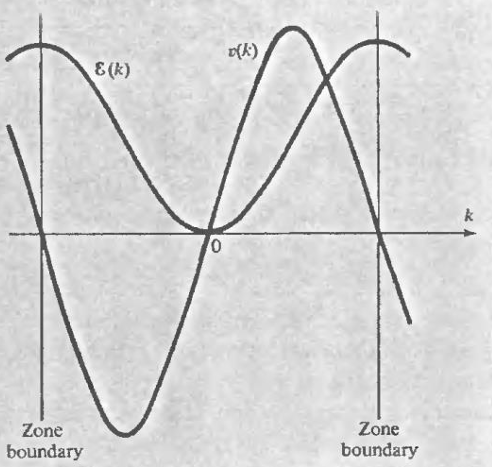
\includegraphics[width=0.4\textwidth]{images/5-Dinamica-Semiclassica/oscilldiBloch.png}
	\caption{Schema delle oscillazioni di Bloch. L'elettrone oscilla avanti e indietro nella banda, a causa della periodicità dell'energia in funzione del vettore d'onda.}
	\label{fig:OscillBloch}
\end{figure}

Nella maggior parte dei materiali reali il tempo d'oscillazione di Bloch è molto più lungo del tempo medio \(\tau\) tra gli scattering, così che questo effetto non è osservabile direttamente. Per evidenziarlo sarebbe necessario utilizzare campioni estremamente puri (con \(\tau\) elevato) oppure materiali in cui la zona di Brillouin sia molto piccola (cioè, con un intervallo \(\Delta k\) ridotto).

\section{Il Modello Semiclassico}
Le seguenti ipotesi semplificano la trattazione della dinamica degli elettroni in un solido:
\begin{enumerate}
    \item \textbf{Banda costante:} La banda \(n\) considerata resta la stessa in presenza del campo esterno; il campo è abbastanza debole da non indurre transizioni inter-banda. (In altre parole, il modello semiclassico non è in grado di descrivere processi di assorbimento che richiederebbero cambi di banda.)
    
    \item \textbf{Dinamica nel \(\vec{k}\)-spazio:} La dinamica del sistema è descritta dalle equazioni:
    \[
    \hbar \frac{\partial k}{\partial t} = e\vec{\nabla}\phi = -e\vec{E} \implies \vec{k}(t) = \vec{k}_0 - \frac{e\,\vec{E}}{\hbar}\, t.
    \]
    \[v_n(\vec{k}(t)) \equiv v\left(\vec{k}_0 -\frac{e\vec{E}}{\hbar}\cdot t \right)  = \frac{1}{\hbar} \frac{\partial \varepsilon_n(\vec{k}(t))}{\partial \vec{k}}\]
    
    \item \textbf{Vettore d'onda come numero quantico:} Il vettore \(\vec{k}\) caratterizza lo stato dell'elettrone, ma non coincide necessariamente con il classico concetto di momento. In un solido il vettore d'onda è definito dalla periodicità del reticolo ed è un numero quantico
    
    \item \textbf{Esclusione di Pauli:} Non è possibile che due elettroni occupino lo stesso stato quantico all'interno della stessa banda \(n\); ciò significa che non possono esistere due elettroni con la stessa posizione \(\vec{r}\) e con vettori d'onda differenti da un vettore reciproco \(\vec{K}\).
    
    \item \textbf{Distribuzione termica:} La distribuzione degli elettroni in funzione dell'energia è data dalla distribuzione di Fermi-Dirac:
    \[
    f\bigl(\varepsilon_n(\vec{k})\bigr)\, \frac{\d\vec{k}}{(2\pi)^3} = \frac{1}{e^{\beta\bigl(\varepsilon_n(\vec{k})-\mu\bigr)}+1}\, \frac{\d\vec{k}}{(2\pi)^3},
    \]
    dove \(\mu\) è il potenziale chimico e \(\beta = 1/(k_BT)\).
    \item \textbf{Perturbazione debole:} Il campo esterno è sufficientemente debole da soddisfare le seguenti condizioni:
    \begin{equation}
        \begin{split}
            eEa &\ll \frac{\bigl[\varepsilon_{\text{gap}}(\vec{k})\bigr]^2}{\varepsilon_F},\\[1mm]
            \hbar\omega_c &\ll \frac{\bigl[\varepsilon_{\text{gap}}(\vec{k})\bigr]^2}{\varepsilon_F},\\[1mm]
            \hbar\omega_c &\ll \varepsilon_{\text{gap}},\\[1mm]
            \lambda &\gg a,
        \end{split}
    \end{equation}
    dove \(a\) è la costante reticolare, \(\varepsilon_{\text{gap}}\) il gap energetico e \(\omega_c\) una frequenza caratteristica determinata dal campo.
\end{enumerate}


\subsection{Massa efficace}
Ora andiamo nel dettaglio della dinamica di un elettrone in un cristallo all'interno di una singola banda. Considero una funzione d'onda di Bloch $\psi_k(\mathbf{r}) = \frac{e^{i\mathbf{k}\cdot \mathbf{r}}}{\sqrt{V}}u_k(\mathbf{r})$ con $u_k(\mathbf{r}+\mathbf{R}) = u_k(\mathbf{r})$. \\
Data l'equazione di Schrodinger: 
\begin{equation}
    \begin{split}
        &H\psi = \varepsilon\psi \hspace{0.2cm}\text{divido da entrambe le parti:}\\
        &e^{-i \vec{k} \cdot \vec{r}}H e^{i \vec{k} \cdot \vec{r}}u_k(\vec{r}) = e^{-i \vec{k} \cdot \vec{r}}\varepsilon e^{+i \vec{k} \cdot \vec{r}}u_k(\vec{r})\\
        &H_k u_k(\vec{r}) = \varepsilon u_k(\vec{r}) \hspace{0.2cm}\text{autostato $u_k$ con stesso autovalore di H}\\
    \end{split}
\end{equation}
Per come si è definita $H_k$ possiamo riscriverla nel seguente modo:
\begin{equation}\label{eqn:Hk}
    \begin{split}
        &H_k \equiv e^{-i \vec{k} \cdot \vec{r}} H( \hat{\mathbf{p}}, \mathbf{r})  e^{i\vec{k} \cdot \vec{r}} = e^{-i\vec{k}\cdot \vec{r}} \left( -\frac{\hbar^2}{2m}\nabla^2+V \right) e^{i\vec{k}\cdot \vec{r}}\\
        &(-i\hbar \vec{\nabla}) e^{i\vec{k}\cdot\vec{r}}u_k(\vec{r}) = e^{i\vec{k}\cdot \vec{r}}(-i\hbar\vec{\nabla}+\hbar \vec{k})u_k(\vec{r}) \hspace{0.2cm}\text{da cui si ottiene:}\\
        &H_k\cdot u_k = e^{-i\vec{k}\cdot\vec{r}} \bigl[\frac{1}{2m}(-i\hbar\vec{\nabla}+\hbar \vec{k})^2+V\bigr]e^{i\vec{k}\cdot\vec{r}}\cdot u_k=\bigl[\frac{1}{2m}(-i\hbar\vec{\nabla}+\hbar \vec{k})^2+V\bigr]\cdot u_k\\
    \end{split}
\end{equation}
e quindi otteniamo:
\[ H( \hat{\mathbf{p}}, \mathbf{r}) \psi_k(\mathbf{r}) = \varepsilon_k\psi_k(\mathbf{r}) \implies H( \hat{\mathbf{p}} + \hbar \mathbf{k}, r) u_k(\mathbf{r}) = \varepsilon_k u_k(\mathbf{r})\]
Mostriamo che per il teorema di Herenfest la velocità è data da:
\[ v = \frac{d\mathbf{r}}{dt} = \frac{i}{\hbar}\left[ H, \mathbf{r}\right] \implies \braket{v_k^{(n)}} = \bra{\psi_k^{(n)}} \frac{d\mathbf{r}(t)}{dt} \ket{\psi_k^{(n)}} = \frac{i}{\hbar}\bra{\psi_k^{(n)}}\left[ H, \mathbf{r}\right]\ket{\psi_k^{(n)}} \]
Calcoliamo $\mathbf{\nabla}_kH_k$:
\begin{equation}
    \begin{split}
        &\mathbf{\nabla}_kH_k=\mathbf{\nabla}_k(e^{-i\vec{k}\cdot\vec{r}}\cdot H \cdot e^{i\vec{k}\cdot\vec{r}})=\\
        &=(-i\mathbf{r})e^{-i\vec{k}\cdot\vec{r}}He^{i\vec{k}\cdot\vec{r}} + e^{-i\vec{k}\cdot\vec{r}} \mathbf{\nabla}_k H e^{i\vec{k}\cdot\vec{r}} + e^{-i\vec{k}\cdot\vec{r}}H(i\mathbf{r})e^{i\vec{k}\cdot\vec{r}} \\
        &\text{il termine centrale si annulla in quanto non dipende da $k$}\\
        &=e^{-i\vec{k}\cdot\vec{r}}(-i\mathbf{r}H) e^{i\vec{k}\cdot\vec{r}} + e^{-i\vec{k}\cdot\vec{r}}(iH\mathbf{r}) e^{i\vec{k}\cdot\vec{r}}\\
        &=i(e^{-i\vec{k}\cdot\vec{r}}[H,\mathbf{r}]e^{i\vec{k}\cdot\vec{r}})\\
    \end{split}
\end{equation}
Da cui la velocità diventa:
\begin{equation}
    \begin{split}
        &\braket{v_k}= \bra{\psi_k} \frac{d\mathbf{r}(t)}{dt} \ket{\psi_k} = \frac{i}{\hbar}\bra{\psi_k}\left[ H, \mathbf{r}\right]\ket{\psi_k} \\
        & =\frac{i}{\hbar}\bra{u_k e^{-i\vec{k}\cdot\vec{r}}}\left[ H, \mathbf{r}\right]\ket{e^{i\vec{k}\cdot\vec{r}}u_k} = \frac{1}{\hbar} \bra{u_k}\mathbf{\nabla}_kH_k\ket{u_k} \hspace{0.2cm}\text{calcolando esplicitamente:}\\
        &=\frac{1}{\hbar} \bigl[\mathbf{\nabla_k} \bra{u_k} H_k \ket{u_k} -  \bra{\nabla_ku_k} H_k \ket{u_k} - \bra{u_k} H_k \ket{\nabla_k u_k}\bigr]\\
        &=\frac{1}{\hbar} \bigl[\mathbf{\nabla_k}\varepsilon(\mathbf{k}) -  \bra{\nabla_ku_k} H_k \ket{u_k} - \bra{u_k} H_k \ket{\nabla_k u_k}\bigr]\\
    \end{split}
\end{equation}
Osserviamo che siccome $\braket{u_k | u_k}=1$ la derivata è nulla per cui:
\begin{equation}
    \begin{split}
    &\bra{\nabla_ku_k} H_k \ket{u_k} = \varepsilon(\mathbf{k}) \braket{\nabla_k u_k | u_k}\\
    &\bra{u_k} H_k \ket{\nabla_k u_k} = \varepsilon(\mathbf{k}) \braket{u_k |\nabla_k u_k} \\
    & \vec{\nabla} \braket{u_k | u_k} = \braket{\vec{\nabla} u_k | u_k} + \braket{u_k | \vec{\nabla} u_k} = 0 \\
    & \implies \braket{\vec{\nabla} u_k | u_k} = - \braket{u_k | \vec{\nabla} u_k} 
    \end{split}
\end{equation}
Quindi il termine $-  \bra{\nabla_ku_k} H_k \ket{u_k} - \bra{u_k} H_k \ket{\nabla_k u_k}$ si elide e da qui si ottiene:
\begin{equation}
    \braket{v_k}= \frac{1}{\hbar} \mathbf{\nabla}_k\varepsilon(\mathbf{k})
\end{equation}
\\\\
Ora posso introdurre il concetto di \textbf{massa effettiva/efficace}, ossia a differenza del elettrone libero, la massa del elettrone non è quella classica ma è un tensore che dipende da k:
\begin{equation}
\begin{split}
    &\hbar \frac{d\mathbf{k}}{dt} = \mathbf{F} = m\mathbf{a}\\
    &\mathbf{a}=\frac{d\braket{v_k^{(n)}}}{dt} = \frac{d}{dt} \biggr(\frac{1}{\hbar}\mathbf{\nabla}_k\varepsilon(\mathbf{k}(t)\biggr)\\
    &=\frac{1}{\hbar}\left( \frac{dk}{dt} \frac{\partial}{\partial k_j} \right) \frac{\partial}{\partial k_i}\varepsilon_k^{(n)} \\
    &= \left( \hbar \frac{dk_j}{dt}\right)\left[ \frac{1}{\hbar^2} \frac{\partial^2 \varepsilon_k^{(n)}}{\partial k_j \partial k_i}\right]= \frac{\mathbf{F}}{m} = \left( \hbar \frac{dk_j}{dt}\right) \frac{1}{\overline{m}_{ij}^{(n)}(k)}
\end{split}
\end{equation} 
Il parametro di proporzionalità tra la forza e la accelerazione non è più uno scalare ma il tensore di massa efficace:
\begin{equation}
    m_{ij} = \left( \frac{1}{\hbar^2} \frac{\partial^2 \varepsilon_k}{\partial k_j \partial k_i}\right)^{-1}
\end{equation}
La massa efficace tiene conto degli effetti che agiscono sugli elettroni quando si muovono all'interno di un reticolo periodico, può essere positiva o negativa a seconda del valore di $\mathbf{k}$ ma questo dipende anche dal tipo di banda, nella banda di conduzione la massa efficace è positiva (elettroni) mentre in quella di valenza è negativa (lacune). Per avere un elettrone molto pesante mi serve una banda molto piatta ($\partial^2\varepsilon$ piccola), solitamente negli isolanti le bande sono piatte (elettroni più "pesanti) ed è per questo che gli elettroni si muovono molto lentamente. 

\section{Probabilità di Scattering}
Consideriamo un sistema in cui avviene lo scattering elastico degli elettroni. Le ipotesi principali sono:
\begin{enumerate}
    \item Lo scattering è elastico, cioè l'energia dell'elettrone rimane invariata.
    \item La probabilità di transizione \(W_{k,k'}\) dall'onda piana di vettore d'onda \(\vec{k}\) a quella di vettore \(\vec{k}'\) è indipendente dalla distribuzione elettronica.
    \item È simmetrica, ovvero \(W_{k,k'} = W_{k',k}\).
    \item Si può utilizzare la regola d'oro di Fermi per calcolare la probabilità di transizione, dato che l'urto provoca una transizione tra stati quantistici.
\end{enumerate}
La probabilità che un elettrone nello stato \(\vec{k}\) venga scatterato, in un intervallo di tempo infinitesimale \(dt\), in un qualsiasi stato nell'elemento di volume \(\d\vec{k}'\) è data da:
\[
\frac{W_{k,k'}\,\d{t}\,\d\vec{k}'}{(2\pi)^3}.
\]
In particolare, utilizzando la regola d'oro di Fermi, il tasso di transizione è:
\[
W_{k,k'} = \frac{2\pi}{\hbar}\, n_i\, \delta\Bigl(\varepsilon(\vec{k})-\varepsilon(\vec{k}')\Bigr)\, \bigl|\langle \vec{k}|U|\vec{k}'\rangle \bigr|^2,
\]
dove:
\begin{itemize}
    \item \(n_i\) è il numero di impurità (o la densità delle stesse) che generano la perturbazione,
    \item \(U\) è il potenziale introdotto dalle impurità, che rompe la periodicità del potenziale cristallino,
    \item La \(\delta\)-di Dirac impone la conservazione dell'energia (scattering elastico).
\end{itemize}
La probabilità totale di scattering per unità di tempo per uno stato \(\vec{k}\) si ottiene integrando su tutti gli stati finali disponibili:
\[
\frac{1}{\tau(\vec{k})} = \int \frac{\d\vec{k}'}{(2\pi)^3}\, W_{k,k'}\,[1-f(\vec{k}')],
\]
dove \(f(\vec{k}')\) è la funzione di distribuzione degli elettroni negli stati finali e il termine \([1-f(\vec{k}')]\) rappresenta la probabilità che lo stato \(\vec{k}'\) sia vuoto (il principio di esclusione di Pauli).\\\\
Per descrivere il processo di scattering nel sistema, si schematizza il flusso in uscita ed in ingresso in un dato stato \(\vec{k}\):

\subsubsection*{Flusso in Uscita}
La probabilità che un elettrone in uno stato \(\vec{k}\) venga scatterato fuori da questo stato (ossia, perda la propria occupazione) è data da:
\[
\left(\frac{df(\vec{k})}{dt}\right)_{\text{out}} = -\frac{f(\vec{k})}{\tau(\vec{k})} = - f(\vec{k}) \int \frac{\d\vec{k}'}{(2\pi)^3}\, W_{k,k'}\,[1-f(\vec{k}')].
\]

\subsubsection*{Flusso in Ingresso}
Analogamente, la probabilità che uno stato \(\vec{k}\) venga occupato da un elettrone proveniente da un altro stato \(\vec{k}'\) è:
\[
\left(\frac{df(\vec{k})}{dt}\right)_{\text{in}} = [1-f(\vec{k})] \int \frac{\d\vec{k}'}{(2\pi)^3}\, W_{k',k}\, f(\vec{k}'),
\]
dove \([1-f(\vec{k})]\) è la probabilità che lo stato \(\vec{k}\) sia vuoto e \(f(\vec{k}')\) è la probabilità che lo stato \(\vec{k}'\) sia occupato.

\subsubsection*{Termine Collisionale}
Combinando i contributi in uscita e in ingresso, il termine collisionale totale diventa:
\begin{equation}\label{eqn:coll}
\begin{split}
\left(\frac{df(\vec{k})}{dt}\right)_{\text{coll}} &= \left(\frac{df(\vec{k})}{dt}\right)_{\text{in}} + \left(\frac{df(\vec{k})}{dt}\right)_{\text{out}} \\
&= [1-f(\vec{k})] \int \frac{\d\vec{k}'}{(2\pi)^3}\, W_{k',k}\, f(\vec{k}') - f(\vec{k}) \int \frac{\d\vec{k}'}{(2\pi)^3}\, W_{k,k'}\,[1-f(\vec{k}')].
\end{split}
\end{equation}
Utilizzando la simmetria \(W_{k,k'} = W_{k',k}\) e riorganizzando i termini, si trova che:
\[
\left(\frac{df(\vec{k})}{dt}\right)_{\text{coll}} = - \int \frac{\d\vec{k}'}{(2\pi)^3}\, W_{k,k'}\,[f(\vec{k}) - f(\vec{k}')].
\]

\subsection{Relaxation Time Approximation}
Per semplificare ulteriormente il problema, si introduce l'approssimazione del tempo di rilassamento. Questa approssimazione si basa su due ipotesi:
\begin{enumerate}
    \item Il tempo medio di collisione \(\tau(\vec{k})\) non dipende dalla funzione di distribuzione stessa $f$, e si assume identico per le collisioni in uscita e in ingresso; in altre parole, la probabilità di transizione da \(\vec{k}\) a \(\vec{k}'\) è simmetrica e può essere caratterizzata da un unico \(\tau(\vec{k})\).
    \item Dopo un tempo sufficientemente lungo, il sistema si porta in equilibrio e la distribuzione degli elettroni assume la forma di \(f_0(\vec{k})\), la distribuzione di Fermi-Dirac locale.
\end{enumerate}
Sostituendo \(f(\vec{k}') \to f_0(\vec{k}')\) nella Eq. \eqref{eqn:coll} e considerando che il sistema tende a portarsi verso l'equilibrio, si definisce il termine collisionale nella \emph{relaxation time approximation} come:
\[
\left(\frac{df(\vec{k})}{dt}\right)_{\text{coll}} = -\frac{f(\vec{k})-f_0(\vec{k})}{\tau(\vec{k})}.
\]

\subsubsection*{Equazione Cinematica (Teorema di Liouville)}
Un altro importante concetto è che, in assenza di collisioni, il teorema di Liouville stabilisce che il volume in spazio delle fasi è conservato. In presenza di scattering, questa condizione non risulta più valida e lo stato della funzione di distribuzione varia secondo:
\begin{equation}\label{eqn:liouville}
f(\vec{k},\vec{r}, t) \to f(\vec{k}+\d\vec{k},\, \vec{r}+d\vec{r},\, t+dt) = f(\vec{k},\vec{r},t) + \left[\frac{\partial f}{\partial t}\right]_{\text{coll}} dt.
\end{equation}
D'altro canto, se consideriamo il movimento degli elettroni in modo semiclassico, un elettrone sottoposto a una forza \(\vec{F}\) subirà una variazione del vettore d'onda data da:
\[
\d\vec{k} = \frac{\vec{F}}{\hbar}\, dt,
\]
e la posizione cambierà di:
\[
d\vec{r} = \vec{v}\, dt,
\]
con \(\vec{v}\) la velocità del pacchetto d'onda. Pertanto, espandendo in serie di Taylor, si ha:
\begin{equation}
\begin{split}
f\Bigl(\vec{k}+\frac{\vec{F}}{\hbar}\,dt,\, \vec{r}+\vec{v}\,dt,\, t+dt\Bigr) &\approx f(\vec{k},\vec{r},t) + \frac{\partial f}{\partial \vec{r}}\cdot \vec{v}\,dt \\
&\quad + \frac{\partial f}{\partial \vec{k}}\cdot \frac{\vec{F}}{\hbar}\, dt + \frac{\partial f}{\partial t}\, dt.
\end{split}
\end{equation}
Equagliando questa espansione con l'evoluzione data da \eqref{eqn:liouville}, si ottiene:
\begin{equation}\label{eqn:boltzmann}
\frac{\partial f}{\partial t} + \vec{v}\cdot \frac{\partial f}{\partial{\vec{r}}}  + \frac{\vec{F}}{\hbar}\cdot  \frac{\partial f}{\partial{\vec{k}}} = -\frac{f - f_0}{\tau},
\end{equation}
che è la forma semplificata dell'equazione di Boltzmann in presenza di collisioni, nella \emph{relaxation time approximation}.

\subsubsection*{Soluzione Semplice in Assenza di Gradiente Spaziale}

Se supponiamo che inizialmente al tempo \(t=0\) il sistema sia disturbato e che la forza esterna sia nulla (ovvero nessun gradiente spaziale) oppure il sistema è isotropo (cosicché \(\nabla_{\vec{r}} f = 0\)), l'equazione \eqref{eqn:boltzmann} si riduce a:
\[
\frac{\partial f}{\partial t} = -\frac{f-f_0}{\tau}.
\]
La cui soluzione è immediata e prende la forma:
\[
f(\vec{k},t) = f_0(\vec{k}) + \left[f(\vec{k},0)-f_0(\vec{k})\right] e^{-t/\tau}.
\]
Questa soluzione mostra che la funzione di distribuzione \(f\) si rilassa esponenzialmente verso la distribuzione di equilibrio \(f_0\) con un tempo caratteristico \(\tau\).

\bigskip
\noindent \textbf{Nota:} Il meccanismo di scattering (spesso dovuto alle impurità) che impedisce l'osservazione completa delle oscillazioni di Bloch è anche la causa della resistività nei materiali. Inoltre, si assume che gli elettroni interagiscano debolmente tra loro, poiché il contributo medio delle interazioni elettrone-elettrone si annulla in un sistema omogeneo (la "nuvola elettronica" appare quasi simmetrica).

\section{Trattazione Semiclassica del Risultato di Drude}
Il modello di Drude descrive la conduzione elettrica in un metallo attraverso la relazione
\[
\vec{J} = \sigma\, \vec{E} \quad \text{con} \quad \sigma = \frac{n\,e^2\,\tau}{m},
\]
dove \(n\) è la densità totale degli elettroni, \(e\) la carica elementare, \(\tau\) il tempo medio di collisione (o tempo di rilassamento) e \(m\) la massa dell'elettrone.\\\\
Nell'approccio semiclassico considerato, si assume che solo gli elettroni in prossimità del livello di Fermi partecipino alla conduzione. In presenza di una perturbazione esterna, la sfera di Fermi in \(\vec{k}\)-spazio inizia a spostarsi e avvengono collisioni (scattering). Gli elettroni, passando in stati vuoti di energia inferiore, subiscono scattering che in media comporta una piccola traslazione della sfera di Fermi, la quale risulta responsabile del flusso di corrente.\\\\
La densità di corrente totale si scrive come
\begin{equation}
    \vec{J} = 2 \int \frac{\d\vec{k}}{(2\pi)^3}\, (-e)\,\vec{v}(\vec{k})\, f(\vec{k}),
\end{equation}
dove il fattore 2 tiene conto della degenerazione per spin, \(\vec{v}(\vec{k})\) è la velocità di gruppo associata a uno stato con vettore d'onda \(\vec{k}\) e \(f(\vec{k})\) è la funzione di distribuzione degli elettroni.\\\\
Si assume che, in presenza di una perturbazione debole, la funzione di distribuzione possa essere scritta come
\[
f(\vec{k}) = f_0(\vec{k}) + f_1(\vec{k}),
\]
dove \(f_0(\vec{k})\) è la distribuzione di equilibrio (la distribuzione di Fermi–Dirac) e \(f_1(\vec{k})\) una piccola variazione dovuta al campo esterno\\
Utilizzando l'approssimazione del tempo di rilassamento, dall'equazione del termine collisionale (vedi la trattazione precedente) in un sistam isotropo e indipendente dal tempo si ottiene:
\[
\frac{1}{\hbar}\,\frac{\partial f_0}{\partial \vec{k}} \cdot \vec{F} = \frac{1}{\hbar}\,\frac{\partial f_0}{\partial \vec{k}} \cdot (-e\,\vec{E}) = -\frac{f(\vec{k})-f_0(\vec{k})}{\tau},
\]
da cui si ricava
\[
f(\vec{k}) = f_0(\vec{k}) + \frac{e\,\tau}{\hbar}\,\frac{\partial f_0}{\partial \vec{k}} \cdot \vec{E} \equiv f_0(\vec{k}) + f_1(\vec{k}) f(\mathbf{k}) \approx f_0(\mathbf{k}+\frac{e\tau}{\hbar}\mathbf{E})\]
per una perturbazione $e\tau \mathbf{E}<<\hbar \mathbf{k}_f$\\
Un'altra forma equivalente, esprimendo la derivata rispetto a \(\vec{k}\) in funzione della derivata rispetto all'energia \(\varepsilon\), è
\[
f_1(\vec{k}) = \frac{e\,\tau}{\hbar}\,\frac{\partial f_0}{\partial \varepsilon}\,\frac{\partial \varepsilon}{\partial \vec{k}} \cdot \vec{E} = e\,\tau\,\frac{\partial f_0}{\partial \varepsilon}\,\vec{v}(\vec{k}) \cdot \vec{E}.
\]
Inserendo questa correzione nella definizione della corrente, la densità di corrente diventa
\[
\vec{J} = \frac{-2e}{(2\pi)^3} \int \d\vec{k}\, \vec{v}(\vec{k})\, \left[f_0(\vec{k}) + f_1(\vec{k})\right].
\]
Il contributo dovuto a \(f_0\) si annulla per simmetria (la sfera di Fermi è isotropa in assenza di campo), perciò rimane
\[
\vec{J} = \frac{-2e}{(2\pi)^3} \int \d\vec{k}\, \vec{v}(\vec{k})\, f_1(\vec{k}).
\]
Sostituendo \(f_1(\vec{k})\) si ottiene
\[
\vec{J} = \frac{-2e}{(2\pi)^3} \int \d\vec{k}\, \vec{v}(\vec{k})\, \left[ e\,\tau\,\frac{\partial f_0}{\partial \varepsilon}\,\vec{v}(\vec{k}) \cdot \vec{E}\right].
\]
Possiamo esprimere questo risultato componente per componente come:
\[
J_\alpha = \frac{e^2}{4\pi^3} \int \d\vec{k}\, \tau\, \left(-\frac{\partial f_0}{\partial \varepsilon}\right)\, v_\alpha(\vec{k})\,\left[\vec{v}(\vec{k}) \cdot \vec{E}\right].
\]
Definendo il tensore di conducibilità mediante \(J_\alpha = \sum_\beta \sigma_{\alpha\beta}\, E_\beta\) e, in un sistema isotropo, scegliendo la direzione del campo \(\vec{E}\) lungo il versore \(\hat{e} = \frac{\vec{E}}{|\vec{E}|}\), si ha
\[
\sigma_0 = \frac{e^2}{4\pi^3} \int \d\vec{k}\, \tau\, \left(-\frac{\partial f_0}{\partial \varepsilon}\right) \, (\hat{e} \cdot \vec{v}(\vec{k}))^2.
\]
In un sistema isotropo la media vale
\[
v_x^2+v_y^2+v_z^2 = v \implies v_x^2 = \frac{v^2}{3} \implies (\hat{e} \cdot \vec{v}(\vec{k}))^2 = \frac{v^2(\vec{k})}{3}.
\]
Inoltre, a basse temperature, la derivata \(-\frac{\partial f_0}{\partial \varepsilon}\) è fortemente concentrata attorno all'energia di Fermi e può essere approssimata con una \(\delta\)-di Dirac:
\[
-\frac{\partial f_0}{\partial \varepsilon} = \delta\bigl(\varepsilon(\vec{k})-\varepsilon_F\bigr).
\]
Utilizzando la definizione della densità degli stati per la banda \(n\)
\[
g_n(\varepsilon) = \frac{1}{(2\pi)^3}\int \delta\bigl(\varepsilon_n(\vec{k})-\varepsilon\bigr)\, \d\vec{k} = \frac{1}{(2\pi)^3} \int_{S_\varepsilon} \frac{\d{S}}{|\nabla_{\vec{k}} \varepsilon(\vec{k})|},
\]
si giunge a
\[
\sigma_0 = \frac{e^2}{3\cdot 4\pi^3} \int \d\vec{k}\, \tau\, v^2(\vec{k})\, \delta\bigl(\varepsilon(\vec{k})-\varepsilon_F\bigr)
= \frac{e^2}{12 \pi^3}\, \tau_F\, v_F^2 \int_{S_F} \frac{\d{S}}{|\vec{\nabla} \varepsilon(\vec{k})|},
\]
dove \(S_F\) è la superficie di Fermi, mentre \(\tau_F\) e \(v_F\) rappresentano il tempo di rilassamento e la velocità a \(k_F\).\\

ricordando che valgono le seguenti relazioni 
\[
 k_F^3 = 3\pi^2\, n \quad v_F = \frac{\hbar k_F}{\overline{m}} \quad \vec{v} = \frac{1}{\hbar}\cdot\nabla\varepsilon(\vec{k}) 
\]
si ottiene la classica formula di Drude:
\[
\sigma_0 = \frac{e^2\,\tau_F}{m^*}\, n.
\]
\vspace{1em}
\section{Lacune}
La conduzione in un metallo è dovuta esclusivamente agli elettroni presenti in bande parzialmente piene. Infatti, le bande completamente piene sono sempre all'equilibrio poiché, nell'approccio semiclassico, il teorema di Liouville garantisce la conservazione del volume nello spazio delle fasi (cioè, la conservazione contemporanea della posizione e del vettore d'onda). Di conseguenza, anche in presenza di campi elettrici e magnetici dipendenti da posizione e tempo, una banda completamente piena resta tale, in quanto le modifiche di stato causate dalla perturbazione si bilanciano esattamente.\\\\
Possiamo infatti esprimere la densità di corrente \(\vec{J}\) come
\begin{equation}
    \vec{J} = (-e) \int \frac{\d\vec{k}}{(4\pi^3)} \, \frac{1}{\hbar}\frac{\partial \varepsilon(\vec{k})}{\partial \vec{k}},
\end{equation}
e l'energia totale come
\begin{equation}
    U = \int \frac{\d\vec{k}}{(4\pi^3)} \, \varepsilon(\vec{k}) \,\frac{1}{\hbar}\frac{\partial \varepsilon(\vec{k})}{\partial \vec{k}}.
\end{equation}
Se l'integrale si estende su tutta la zona di Brillouin e la funzione \(\varepsilon(\vec{k})\) riguarda una banda completamente piena, i contributi relativi alle velocità con segni positivi e negativi si cancellano (perché la funzione è periodica e simmetrica), e quindi entrambi gli integrali risultano nulli. Questo implica che le bande piene non contribuiscono alla conduzione elettrica.\\\\
La conduzione è dunque determinata esclusivamente dalle "quasi particelle" presenti in bande parzialmente piene, dove esistono degli stati vuoti (dette anche \emph{lacune}) in cui gli elettroni possono muoversi.

\subsection*{Concetto di Lacuna}

Il termine \emph{lacuna} indica uno stato non occupato in una banda che, altrimenti, sarebbe completamente piena. Le lacune non sono particelle elementari, ma quasiparticelle che nascono dall'azione collettiva degli elettroni. Consideriamo i seguenti punti:
\begin{itemize}
    \item Quando la banda è completamente piena, la somma vettoriale dei vettori d'onda degli elettroni è uguale a zero: \(\sum_i \vec{k}_i = 0\).
    \item Se si rimuove un elettrone dalla banda (ad es. un elettrone con vettore d'onda \(\vec{k}_e\) viene promosso in una banda di conduzione), la somma dei vettori d'onda degli elettroni rimasti diventa
    \[
    \sum_i \vec{k}_i = -\vec{k}_e,
    \]
    e dunque, per mantenere la condizione di equilibrio (la somma totale deve restare zero), il vettore d'onda associato allo stato vuoto (la lacuna) deve essere:
    \[
    \vec{k}_h = -\vec{k}_e.
    \]
\end{itemize}
Questo procedimento è una conseguenza del fatto che, essendo un effetto collettivo, la definizione della lacuna nasce dalla differenza fra l'insieme degli stati occupati e la condizione di band complete. In altre parole, se scriviamo:
\[
\sum_i \vec{k}_i = \sum_{\text{occupati}} \vec{k}_i + \sum_{\text{non occupati}} \vec{k}_i = 0,
\]
allora la mancanza di un elettrone in un particolare stato si traduce in un contributo netto uguale al vettore \(-\vec{k}_e\).

\subsection*{Energia della Lacuna}
Per quanto riguarda l'energia, immaginiamo di avere una banda di valenza completamente piena e una banda di conduzione completamente vuota, come illustrato in Figura~\ref{fig:lacune1}. Se, promuovendo un elettrone dallo stato \(\vec{k}_e\) della banda di valenza (VB) a uno stato della banda di conduzione (CB) mediante l'assorbimento di un fotone (con \(\hbar\omega > E_g\), dove \(E_g\) è il gap energetico), si crea nello stesso momento una lacuna nella banda di valenza, la reazione è:
\[
e(\text{VB}) + \text{fotone}\, (\hbar\omega > E_g) \to e(\text{CB}) + h(\text{VB}).
\]
Quando la banda di valenza è piena, la somma totale dei vettori d'onda è nulla:
\[
\vec{k}_{\text{band}} = \sum_i \vec{k}_i = 0.
\]
Pertanto, rimuovendo un elettrone con vettore \(\vec{k}_e\) si ottiene che il vettore d'onda della lacuna è:
\[
\vec{k}_h = -\vec{k}_e.
\]
Per quanto riguarda l'energia, convenzionalmente si prende $E_e(\text{VB}) < 0$,
\[ E_e(\text{VB}) + \hbar\omega = E_e(\text{CB})\]
Ma
\[\hbar\omega = E_e(\text{CB}) + E_h(\text{VB}) \]
Da cui si ricava 
\[E_e(\text{VB})+ \cancel{E_e(\text{CB})} + E_h(\text{VB}) = \cancel{E_e(\text{CB})}
    \implies E_h(\text{VB}) = - E_e (\text{VB})\]
Questo risultato esprime il fatto che, dal punto di vista delle lacune, lo spazio e l'energia si conservano: per ridurre l'energia, l'elettrone in banda di conduzione tenderà a scendere (per minimizzare l'energia totale) mentre la lacuna, per effetto opposto, tenderà a spostarsi verso energie più elevate nella banda di valenza.


\subsection*{Massa Efficace e Velocità della Lacuna}
La massa efficace della lacuna si ricava dalla seconda derivata dell'energia rispetto al vettore d'onda. Formalmente, si scrive:
\[
\frac{1}{m_h^*} = \frac{1}{\hbar^2} \frac{\partial^2 E_h(\vec{k}_h)}{\partial k_i^{(h)} \partial k_j^{(h)}}.
\]
Utilizzando la relazione \(E_h(\vec{k}_h) = -E_e(\vec{k}_e)\) e \(\vec{k}_h = - \vec{k}_e\), si ottiene:
\[
\frac{1}{m_h^*} = -\frac{1}{\hbar^2} \frac{\partial^2 E_e(\vec{k}_e)}{\partial k_i^{(e)} \partial k_j^{(e)}}.
\]
Quindi, la massa efficace della lacuna risulta essere:
\[
m_h^* = - m_e^*.
\]
Analogamente, la velocità di gruppo della lacuna è definita come
\[
v_h(\vec{k}_h) = \frac{1}{\hbar} \frac{\partial E_h(\vec{k}_h)}{\partial \vec{k}_h}.
\]
Utilizzando la relazione \(E_h(\vec{k}_h) = -E_e(\vec{k}_e)\) e \(\vec{k}_h = -\vec{k}_e\), si trova:
\[
v_h(\vec{k}_h) = \frac{1}{\hbar} \frac{\partial E_e(\vec{k}_e)}{\partial \vec{k}_e} = v_e(\vec{k}_e).
\]
Pertanto, la velocità della lacuna coincide con quella dell'elettrone, mentre la massa efficace ha il segno opposto.

\subsection*{Comportamento in Presenza di una Forza Esterna}

Consideriamo l'effetto di una forza esterna sul sistema. Dal punto di vista della lacuna, l'evoluzione del vettore d'onda è governata da
\[
\hbar \frac{\d\vec{k}_h}{dt} = q_h \left[\vec{E} + \vec{v}_h \times \vec{B}\right],
\]
mentre dal punto di vista dell'elettrone:
\[
\hbar \frac{d\vec{k}_e}{dt} = q_e \left[\vec{E} + \vec{v}_e \times \vec{B}\right],
\]
dove \(q_e = -e\). Poiché \(\vec{k}_h = -\vec{k}_e\), derivando rispetto al tempo si ottiene:
\[
- \hbar \frac{d\vec{k}_e}{dt} = q_h \left[\vec{E} + \vec{v}_e \times \vec{B}\right].
\]
La relazione per l'elettrone è:
\[
\hbar \frac{d\vec{k}_e}{dt} = -e \left[\vec{E} + \vec{v}_e \times \vec{B}\right].
\]
Le due equazioni saranno compatibili se:
\[
q_h = -q_e = +e.
\]
Questo conferma che, dal punto di vista dinamico, la lacuna si comporta come una particella con carica positiva \(+e\).

\subsection*{Conclusioni sul Ruolo delle Lacune}
La conduzione elettrica è determinata dal riempimento delle bande:
\begin{enumerate}
    \item \textbf{Metalli:} Presentano almeno una banda parzialmente piena, in cui la conduzione è dovuta principalmente agli elettroni.
    \item \textbf{Semimetalli:} Hanno il livello di Fermi posizionato in una regione con densità di stati molto bassa, e quindi pochi portatori contribuiscono al trasporto.
    \item \textbf{Semiconduttori:} La banda di valenza è quasi piena e la banda di conduzione quasi vuota; la conduzione avviene promuovendo elettroni dalla banda di valenza alla banda di conduzione, generando contemporaneamente lacune.
    \item \textbf{Isolanti:} Presentano una banda di valenza completamente piena e una banda di conduzione vuota, separati da un gap energetico elevato, rendendo difficile l'eccitazione di elettroni.
\end{enumerate}
Possiamo vedere anche il comportamento della densità di corrente integrando sull'intera zona di Brillouin:
\[
j = \int_{\text{BZ}} \frac{\d\vec{k}}{(4\pi^3)}\, (-e)\, v(\vec{k}) = 0,
\]
perché, in una banda completamente piena, le componenti della corrente dovute agli stati occupati si annullano per simmetria. Possiamo scrivere questo risultato come:
\[
0 = \int_{\text{occupati}} \frac{\d\vec{k}}{(4\pi^3)}\, (-e)\, v(\vec{k}) + \int_{\text{non occupati}} \frac{\d\vec{k}}{(4\pi^3)}\, (-e)\, v(\vec{k}).
\]
Da qui si può ricavare che:
\[
\int_{\text{non occupati}} \frac{\d\vec{k}}{(4\pi^3)}\, (-e)\, v(\vec{k}) = \int_{\text{occupati}} \frac{\d\vec{k}}{(4\pi^3)}\, (+e)\, v(\vec{k}),
\]
il che significa che la corrente prodotta se si trascurano gli elettroni negli stati occupati è equivalente a quella prodotta dalle lacune, che agiscono come portatori con carica \(+e\).

